\chapter{Importing and Exporting}
\label{ch:importexport}

\ccprod{} reads and writes two foreign formats: comma-separated text
(\fname{.CSV}) and Excel workbooks (\fname{.XLSX}). Both are interchange
formats. Once a file has been imported the workbook lives entirely in
\ccprod's own engine; there is no link back to the file it came from.

\begin{cctable}{Command}{Key}{2.2in}{2.62in}
\menupath{File > Import} & \key{F7} \\
\menupath{File > Export} & \key{F8} \\
\end{cctable}

\section{Importing}
\index{import}

\key{F7} lists every file in the directory ending \fname{.XLSX} or
\fname{.CSV}, in the same browsable list \menupath{Open} uses --- so an import
can be picked out of a subdirectory. Choose
one and \ccprod{} decides what to do with it by its name: \fname{.XLSX} goes
through the Excel importer, anything else through the CSV reader.

\begin{ccnote}
The box is titled \msg{Open}, not \msg{Import}. It is the same dialogue.
\end{ccnote}

The two importers differ in one large respect: \textbf{a CSV is read into the
worksheet you are on; an XLSX replaces the entire workbook.} Both start at
\cellref{A1}.

\section{Importing a CSV}
\index{CSV!import}

The file is read in at \cellref{A1}, whatever the cursor was on, and fills
down and right from there. Anything already in those cells is overwritten;
cells outside the block are left alone, so importing a small CSV into a large
sheet replaces a corner of it rather than the whole thing.

Each field is interpreted exactly as though you had typed it into that cell:
numbers become numbers, \lit{TRUE} and \lit{FALSE} become booleans, a field
beginning \lit{=} becomes a formula, and \lit{007} becomes the number 7.

\begin{cctable}{The reader accepts}{Detail}{1.75in}{3.07in}
Commas & And only commas. There is no delimiter detection and no way to ask
for semicolons or tabs. \\
Any line ending & Carriage return, line feed, or both. \\
Quoted fields & A field starting with \lit{"} runs to the closing quote;
\lit{""} inside it is one literal quote. \\
Rubbish after a closing quote & Discarded rather than treated as an error,
because real files contain it. \\
A missing final newline & The last row still arrives. \\
\end{cctable}

An empty quoted field, \lit{""}, leaves the cell empty rather than storing an
empty piece of text. Empty fields still take up their column position, so
values after a gap stay in the right column.

\begin{cccaution}
A field is cut off at \textbf{ninety-five characters}, silently. Long text in a
CSV arrives shortened with no warning of any kind.
\end{cccaution}

When the import finishes, a box reports what happened:

\begin{ccfigure}
\ccscreenscale{1.15}
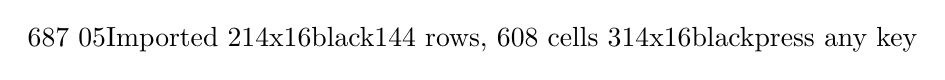
\begin{tikzpicture}
\node[inner sep=0pt,anchor=north west] (ir) at (0,0) {%
\ccscreenbegin{68}{7}
  \ccdlgbox{0}{5}{Imported}
  \cctext{2}{14}{x16black}{144~rows,~608~cells}
  \cctext{3}{14}{x16black}{press~any~key}
\ccscreenend
};
\end{tikzpicture}
\caption{The result of a CSV import}
\label{fig:csvresult}
\end{ccfigure}

If an empty pair of brackets \msg{()} appears after the counts, the import ran
off the edge of the worksheet or hit the sixteen-thousand-cell limit and some
of the file was left out. The brackets are empty because of a fault in the
program --- see \emph{Reading the note} below --- but they are reliable as a
warning sign.

\section{Exporting a CSV}
\index{CSV!export}

\key{F8} asks for a name. Any name that does not end \fname{.XLSX} produces a
CSV.

\begin{ccsteps}
\item Fields are separated by commas and lines end with carriage return and
line feed, which is what every other spreadsheet writes.
\item A field is quoted only if it needs to be --- if it contains a comma, a
quote, or a line ending. An embedded quote is doubled.
\item The whole used range of the current worksheet is written, empty cells
included, so the columns line up.
\item \textbf{Values are written, not formulas.} A cell holding
\fml{=SUM(B2:B7)} exports as \lit{13388.2}.
\item Cells are written as they are \emph{displayed}, so a currency-formatted
cell exports as \lit{\$8400.00}, dollar sign and all.
\end{ccsteps}

\begin{ccnote}
Only the current worksheet is exported. A CSV file has no way to hold more than
one, so the other fifteen are not written and you are not told.
\end{ccnote}

\section{Importing an XLSX}
\index{XLSX!import}

An \fname{.XLSX} file is a compressed archive of documents. \ccprod{} opens the
archive, expands each part it needs into memory and reads it --- five separate
passes, on an eight-megahertz processor, with a trip to the card between each
one. It is slow, and it says so:

\begin{ccfigure}
\ccscreenscale{1.15}
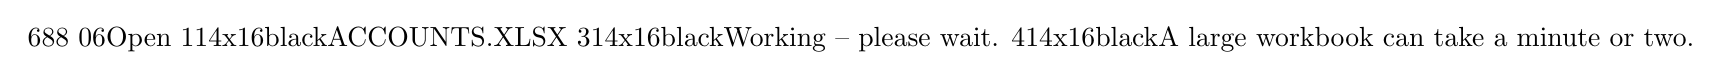
\begin{tikzpicture}
\node[inner sep=0pt,anchor=north west] (bz) at (0,0) {%
\ccscreenbegin{68}{8}
  \ccdlgbox{0}{6}{Open}
  \cctext{1}{14}{x16black}{ACCOUNTS.XLSX}
  \cctext{3}{14}{x16black}{Working~--~please~wait.}
  \cctext{4}{14}{x16black}{A~large~workbook~can~take~a~minute~or~two.}
\ccscreenend
};
\end{tikzpicture}
\caption{The busy box shown throughout an import}
\label{fig:busybox}
\end{ccfigure}

The box does not animate and does not show progress. It stays exactly as it is
until the import finishes.

\begin{ccnote}
For a sense of scale: five hundred days of stock prices in six columns --- about
three thousand cells --- takes \textbf{fifty-one seconds} to open as an
\fname{.XLSX} and \textbf{seventeen seconds} as a \fname{.X16S}. If you are
going to use a workbook more than once, import it and then save it in
\ccprod's own format.
\end{ccnote}

\subsection{What comes across}

\begin{cctable}{Feature}{Imported}{2.1in}{2.72in}
All worksheets & Yes, up to sixteen \\
Worksheet names & Yes, first 31 characters \\
Numbers & Yes \\
Text & Yes, from shared strings or inline \\
Dates & Yes, as date cells if the style says so \\
\msg{TRUE} and \msg{FALSE} & Yes \\
Error values & Yes \\
Number formats & Yes, mapped onto \ccprod's eight \\
Column widths & Yes \\
Formulas & Yes, if \ccprod{} can compile them --- see below \\
\end{cctable}

\subsection{What does not}

Nothing in an \fname{.XLSX} is treated as an error just because \ccprod{} does
not understand it. Unrecognised content is stepped over, so a workbook with a
chart in it still opens --- without the chart.

\begin{cctable}{Feature}{What happens}{2.1in}{2.72in}
Charts, pivot tables & Not read. Gone. \\
Fonts, fills, borders, colours & Read past. Only the number format is taken;
even bold is not imported. \\
Merged cells & Not handled \\
Conditional formatting, validation & Not handled \\
Comments, hyperlinks, images, macros & Not handled \\
Row heights & Not handled \\
Frozen panes, print settings, filters & Not handled \\
Defined names & Not handled \\
Worksheets past the sixteenth & Skipped, and reported \\
ZIP64 archives & Refused \\
Password-protected files & Refused \\
\fname{.XLS} files & Refused. They are not archives. \\
\end{cctable}

\subsection{Formulas that will not compile}

\ccprod{} has fourteen functions. An Excel workbook will have formulas it
cannot translate --- a \fn{VLOOKUP}, a \fn{SUMIF}, anything with a named range.

Those cells are not left empty and are not marked with an error. They keep the
value Excel last calculated for them, so the workbook looks right and adds up
right. What they will not do is \emph{change} when their inputs change.

The result box says so, with a note in brackets after the counts:

\begin{ccfigure}
\ccscreenscale{1.15}
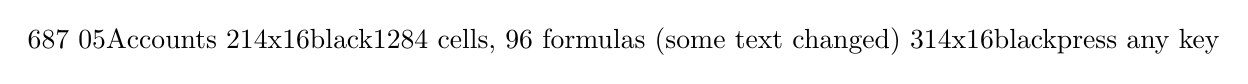
\begin{tikzpicture}
\node[inner sep=0pt,anchor=north west] (xr) at (0,0) {%
\ccscreenbegin{68}{7}
  \ccdlgbox{0}{5}{Accounts}
  \cctext{2}{14}{x16black}{1284~cells,~96~formulas~(some~text~changed)}
  \cctext{3}{14}{x16black}{press~any~key}
\ccscreenend
};
\end{tikzpicture}
\caption{The result of an XLSX import. The title is the first worksheet's name}
\label{fig:xlsxresult}
\end{ccfigure}

\begin{cccaution}
This is the most dangerous thing in the program, and it is dangerous precisely
because it looks like it worked. A cell showing a total that no longer responds
to the numbers above it is indistinguishable, on screen, from one that does.
After importing an Excel workbook, check the formula bar on the cells that
matter.
\end{cccaution}

\begin{ccnote}
An imported formula reads with a leading \lit{=} in the formula bar, the same
as one you typed, and copies and re-edits as a formula.

That is worth saying because an \fname{.XLSX} does not store the \lit{=}: the
file holds \lit{SUM(B1:B9)}, and \ccprod{} puts the \lit{=} back as it reads
it. Earlier versions did not, and an imported formula that was copied or
re-edited turned into a \emph{label} reading \lit{SUM(B1:B9)} --- text that
looked almost right and calculated nothing.
\end{ccnote}

\subsection{Reading the note}

\begin{cccaution}
\textbf{The counts on a result box are right. The note in brackets after them
is not.} The program picks the wrong phrase from its list --- it is off by one
--- so the words that appear describe the \emph{previous} condition, and one
case comes out as an empty pair of brackets.

Read the note by what it means here, not by what it says:

\begin{cctable}{What appears}{What it actually means}{1.42in}{3.13in}
\msg{()} & A limit was reached --- cells, formulas, shared strings or styles
--- and the rest of the file was not imported. \\
\msg{(some did not fit)} & The file contained characters with no equivalent in
the Commander X16's character set. They were replaced with \lit{?}. \\
\msg{(some text changed)} & Some formulas could not be compiled and are held as
fixed values. \\
No brackets at all & Nothing went wrong. \\
\end{cctable}

The phrase \msg{some formulas kept as values} is in the program but can never
appear on screen.
\end{cccaution}

The second count is not always the same thing either. If the file had more than
sixteen worksheets, the box reports how many were \emph{skipped}; otherwise it
reports how many formulas came across.

\begin{cctable}{Reads}{Means}{2.1in}{2.72in}
\msg{1284 cells, 96 formulas} & All the worksheets fitted; 96 formulas were
compiled. \\
\msg{1284 cells, 2 more sheets skipped} & The file had eighteen worksheets and
two were left behind. \\
\end{cctable}

\subsection{When an import fails outright}

The workbook in memory is cleared \emph{before} the import begins, so a failure
leaves you with an empty workbook rather than a half-replaced one. Save your
work before importing.

\begin{cctable}{Message}{Means}{1.85in}{2.97in}
\msg{Damaged or unrecognised file} & Not a ZIP archive; or the archive has no
\fname{xl/workbook.xml}, which means it is not an \fname{.XLSX} at all; or a
part did not expand to the size the archive promised. \\
\msg{Out of memory} & There was not enough banked RAM to stage the file. See
below. \\
\msg{File not found} & The archive is well-formed but does not contain the
worksheet its own index points at. \\
\end{cctable}

\subsection{How big a file can be imported}
\index{XLSX!size limits}

The worksheet's XML has to be held in banked memory in its compressed form
\emph{and} its expanded form at the same time, with the growing cell store
beside them. One part may be at most 128K expanded.

That is a real limit and it arrives sooner than the cell count does. Five
hundred days of six-column data --- 118K of XML --- imported with two megabytes
still free. Two thousand days --- 478K of XML --- was refused on a machine with
1.98M free. On data of that shape the practical ceiling is around three thousand
cells, and a 256K worksheet cannot be imported on a 512K machine at all.

\section{Exporting an XLSX}
\index{XLSX!export}

\key{F8} and a name ending \fname{.XLSX}, in any case.

Every worksheet is written, each as its own part. Text goes inline rather than
into a shared string table. Formulas are written twice --- as the formula and
as the value \ccprod{} calculated --- so that a program reading the file sees
the right number whether or not it recalculates.

\begin{cctable}{Written}{Not written}{2.1in}{2.72in}
All worksheets and their names & Colours \\
Numbers, text, dates, booleans, errors & Alignment \\
Formulas, with their cached values & Frozen panes, row heights \\
Number formats & Merged cells, charts, defined names \\
Bold & A modification date --- files show as 1980 \\
Column widths that differ from the default & \\
\end{cctable}

\begin{ccnote}
\textbf{Nothing is compressed.} Every part of the archive is stored, not
deflated, because a DEFLATE compressor would not fit in the space available. A
workbook that Excel would write as a 40K file comes out of \ccprod{} at about
200K. It is a perfectly valid \fname{.XLSX} --- Excel, LibreOffice and Google
Sheets all open it --- it is simply five times the size.
\end{ccnote}

If an export fails part way through, the file left on the card is not a valid
archive at all rather than one that opens with content missing. That is
deliberate: a file that will not open is a better outcome than one that opens
and is wrong.
